\documentclass{article}

\usepackage{graphicx}
\usepackage{adjustbox}
\usepackage{polski}
\usepackage{float}
\usepackage{lscape}
\usepackage[margin=2.5cm]{geometry}

\setlength{\parindent}{0pt}

\title{Raport - czynniki wpływające na zarobki w branży IT}
\author{Michał Puchyr}

\begin{document}

\begin{titlepage}


    \begin{center}

        \LARGE \textsc{Politechnika Wrocławska}\\
        \vspace*{0.2cm}
        \Large \textsc{Wydział Informatyki i Telekomunikacji}\\
        \vspace*{0.4cm}
        \centering
\includegraphics[width=0.2\textwidth]{WITlogo.png}\\
        \vspace*{0.2cm}
        \vspace*{2cm}

        \centerline{\rule{\textwidth}{1.2pt}}
        \vspace{0.4cm}
        \Huge\textbf{Metody i Systemy Decyzyjne}
        \centerline{\rule{\textwidth}{1.2pt}}
        \vspace{1cm}
        \LARGE Raport - "Co wpływa na wynagrodzenie w branży IT?"\\
        \vspace{3.5cm}
        \textsc{Autor}\\
        \vspace{0.2cm}
        \textbf{Michał Puchyr}\\
        \vspace{0.1cm}
        \Large nr albumu: \textbf{272733}\\
        \vspace{0.1cm}
        kierunek: \textbf{Informatyka Stosowana}

        \vspace*{\fill}
        \Large \textit{\today}

    \end{center}
\end{titlepage}


\section{Problem badawczy}

\textbf{Problem badawczy:} Jakie czynniki najbardziej wpływają na zarobki w branży IT w Polsce?

Celem niniejszego raportu jest zbadanie czynników wpływających na zarobki w branży IT. Rozwój technologii informatycznych sprawia, że specjaliści IT
są jednymi z najbardziej poszukiwanych pracowników na rynku pracy. W związku z tym że, zarobki informatyków są bardzo zróżnicowane i zależne od wielu czynników,
w niniejszym raporcie zostaną przedstawione wyniki badań dotyczące wynagrodzenia informatyków w Polsce oraz czynników, które wpływają na ich wysokość.


\section{Dane badawcze}

Dane potrzebne do przeprowadzenia analizy zostały pobrane z portali NoFluffJobs oraz Pracuj.pl.

\begin{itemize}
    \item Nazwa oferty
    \item Nazwa firmy (pracodawcy)
    \item Technologie (języki programowania i narzędzia)
    \item Poziom doświadczenia (trainee, junior, mid, senior, expert)
    \item Lokalizacja
    \item Zarobki (widełki płacowe - minimalne i maksymalne)
    \item Czy praca jest zdalna
\end{itemize}

\bigskip

Do celów analitycznych zostało pobranych 2859 ofert pracy.
Niestety nie wszystkie oferty zawierały informacje o zarobkach, dlatego zostały one odfiltrowane.

\begin{figure}[h]
    \centering
    \begin{minipage}{0.45\textwidth}
        \centering
        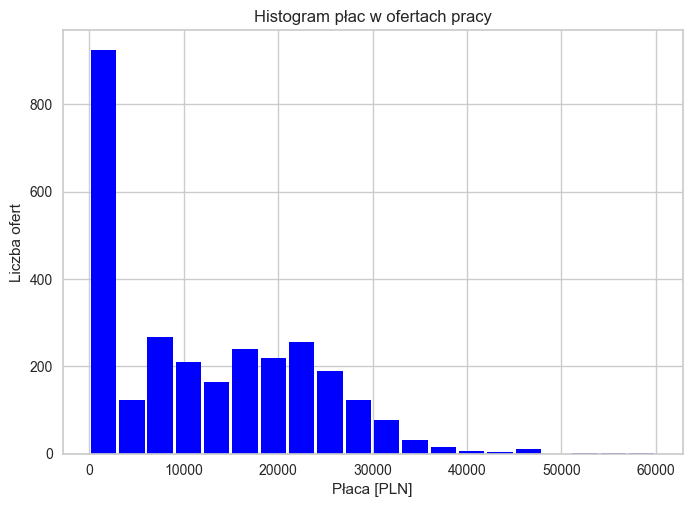
\includegraphics[width=\textwidth]{img/hist_zarobki_z_zerami.png}
    \end{minipage}
    \hfill
    \begin{minipage}{0.45\textwidth}
        \centering
        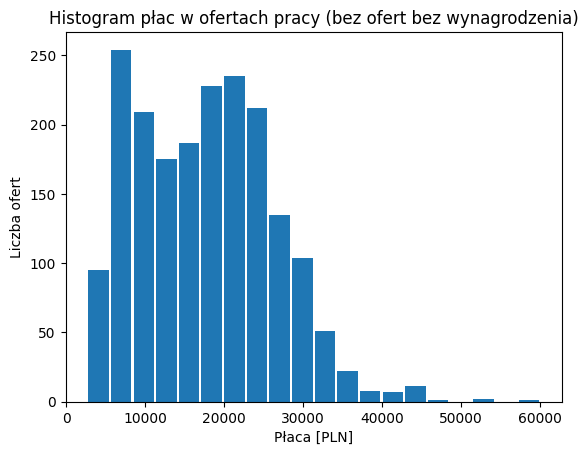
\includegraphics[width=\textwidth]{img/hist_zarobki_bez_zer.png}
    \end{minipage}
\end{figure}

W procesie czyszczenia danych, oferty pracy, które nie zawierały informacji o wynagrodzeniu, miały wartości zerowe w kolumnie zarobków.
\textbf{Brak danych o zarobkach występuje w około 32\% ofertach pracy}.
\medskip

Lokalizacje ofert pracy, których liczba wystąpień była mniejsza bądź równa 5, zostały
zgrupowane do jednej kategorii - 'Other' tak aby nie wpłynęły na czytelność wykresów i analizy danych.
Lokalizacje zza granicy zostały zgrupowane do jednej kategorii - 'Abroad'.

Poziomy doświadczenia z ofert pracy z portalu Pracuj.pl zostały przekształcone na poziomy zgodne z ofertami z portalu NoFluffJobs w celu ujednolicenia danych.
Poziomy doświadczenia zostały przekształcone na: \textit{trainee, junior, mid, senior, expert}.

Nie każda oferta zawierała informacje o języku naturalnym oraz o technologii wymaganej do pracy. Wartości takie w bazie danych posiadają wartość null.
W przypadku użycia kodowania one-hot, wartości null są ignorowane.

Oferty pracy z brakiem informacji o wynagrodzeniu zostały odzucone w dalszej analizie ze względu na brak możliwości ich uzupełnienia i wykorzystania do modelowania.

\begin{table}[H]
    \centering
    \begin{adjustbox}{width=1.1\textwidth}
        \begin{tabular}{|c|c|c|c|c|c|c|c|c|c|c|}
            \hline
            \textbf{Id} & \textbf{Name}     & \textbf{SalaryFrom} & \textbf{SalaryTo} & \textbf{ExpLevel} & \textbf{Category} & \textbf{JobLanguage} & \textbf{Location} & \textbf{IsRemote} & \textbf{Technology} & \textbf{Company}  \\ \hline
            125         & Ework Group       & 18480.00            & 29400.00          & Senior            & erp               &                      & Kraków            & false             &                     & Ework Group       \\ \hline
            126         & ROCKWOOL          & 0.00                & 0.00              & Mid               & support           &                      & Poznan            & false             &                     & ROCKWOOL          \\ \hline
            127         & Omni Calculator   & 7300.00             & 9600.00           & Mid               & marketing         &                      & Remote            & true              &                     & Omni Calculator   \\ \hline
            150         & Devire Sp. z o.o. & 28560.00            & 35280.00          & Mid               & backend           & pl, en               & Warszawa          & false             & Java                & Devire Sp. z o.o. \\ \hline
            151         & ITDS              & 14700.00            & 23100.00          & Senior            & fullstack         & pl                   & Warszawa          & false             & .NET                & ITDS              \\ \hline
        \end{tabular}
    \end{adjustbox}
    \caption{Przykładowy wycinek danych na podstawie których przeprowadzono analizę}
    \label{tab:oferty}
\end{table}

\section{Analiza danych}

\begin{table}[h!]
    \centering
    \begin{tabular}{|c|c|c|c|c|c|c|c|c|}
        \hline
                      & Średnia  & Mediana  & Odchylenie std. & Min     & 25\%     & 50\%     & 75\%     & Maks     \\
        \hline
        Zarobki [PLN] & 17637.34 & 17500.00 & 8578.94         & 2664.00 & 10000.00 & 17500.00 & 23520.00 & 60000.00 \\
        \hline
    \end{tabular}
    \caption{Statystyki opisowe zarobków programistów}
    \label{tab:zarobki}
\end{table}

Mediana wysokości płacy analizowanych ofert pracy wynosi 17\,500 PLN, a średnia 17\,637.34 PLN.

Odchylenie standardowe wynosi 8\,578.94 PLN, co oznacza, że zarobki w branży IT są bardzo zróżnicowane.
Najwięcej ofert pracy możemy znaleźć w przedziale od 7\,500 PLN do 23\,520 PLN.
Z wykresu możemy również odczytać, że oferty pracy z wynagrodzeniem powyżej 35\,000 PLN są rzadkością.

Możemy zatem przyjąć, że zarobki w branży IT mieszczą się w przedziale od 3\,000 PLN - 40\,000 PLN.

\begin{center}
    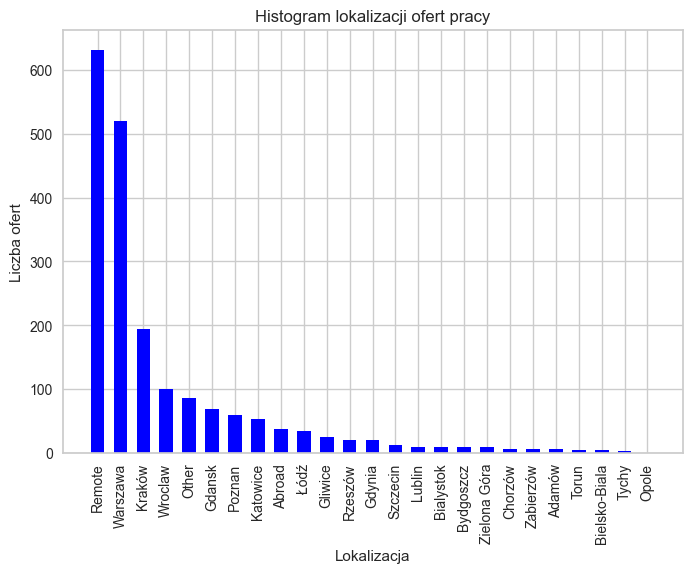
\includegraphics[scale=0.6]{img/location_hist.png}
\end{center}

Najpopularniejszą "lokalizacją" pracy dla programistów jest praca zdalna.
Praca zdalnych jako lokalizacja występuje w 32\% ofert pracy. Jej wpływ na wynagrodzenie
zostanie zbadany w dalszej części raportu.
W przypadku lokalizacji pracy stacjonarnej najwięcej ofert pracy pochodzi z odpowiednio z
Warszawy, Krakowa, Wrocławia, Gdańska i Poznania co pokrywa się z wielkością tych miast
pod względem liczby mieszkańców.
Do raportu zostały również uwzględnione oferty pracy zza granicy, liczba takich ofert
w porównaniu do ofert z Polski jest znikoma, stanowią one zaledwie 2\% wszystkich ofert,
w związku z czym zostały one wrzucone do jednej kategorii - "Abroad".

\begin{center}
    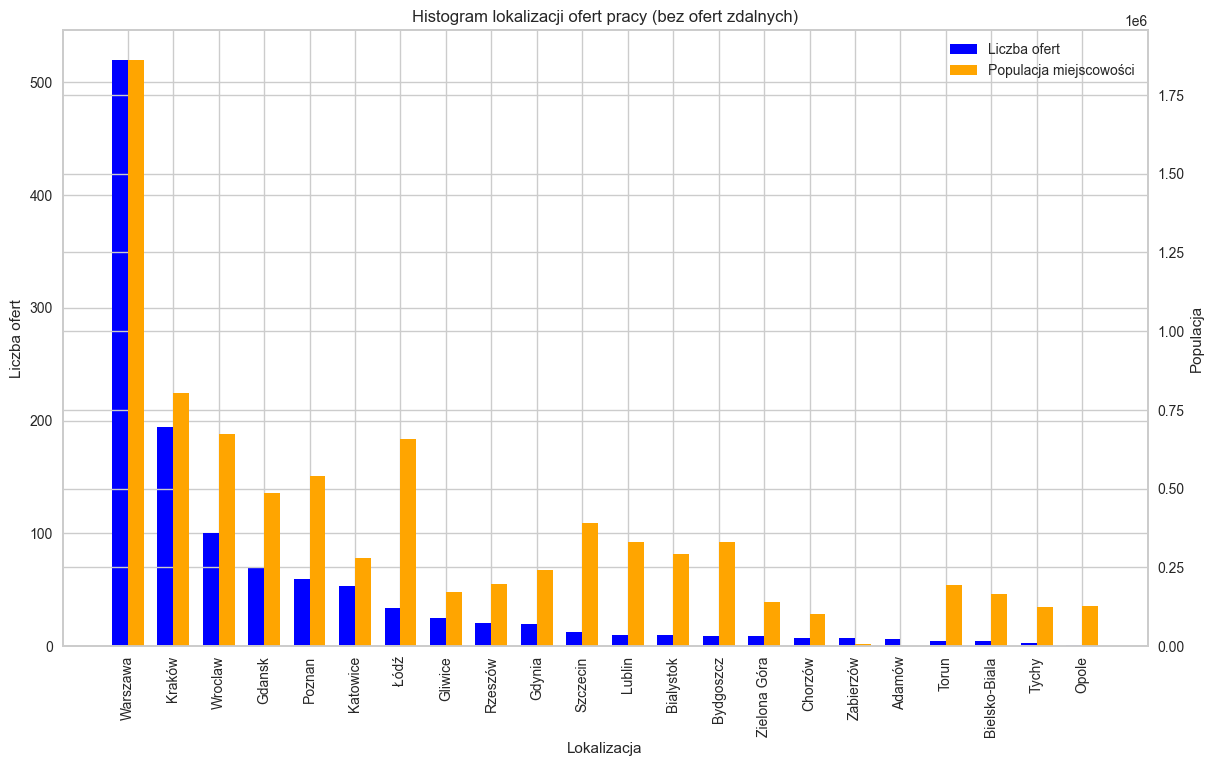
\includegraphics[scale=0.5]{img/location_with_pop.png}
\end{center}

Jeśli weźmiemy pod uwagę do lokalizacji ofert liczbę mieszkańców w danym mieście
możemy zauważyć, że liczba mieszkańców nie zawsze bedzie oznaczać większą liczbę ofert pracy.

Punktem odniesienia jest Warszawa, gdzie słupek z liczbą ofert pracy jest na równi ze spłupkiem
liczby mieszkańców.
Proporcja wysokości słupków liczby ofert pracy i ludności dla reszty miast jest odniesiona
bezpośrednio do Warszawy.

Wiedząc to, możemy wyczytać, że Wrocław jest miastem, które jak na swoją liczbę mieszkańców
powinno mieć więcej ofert pracy tak aby dorównać Warszawie przy swojej liczbie mieszkańców.

Aby ułatwić analizę ludności i liczby ofert możemy wyliczyć proporcje liczby ofert pracy do liczby mieszkańców.
Wartość ta pozwoli na zobrazowanie, w którym mieście jest największe zagęszczenie ofert pracy.


\begin{center}
    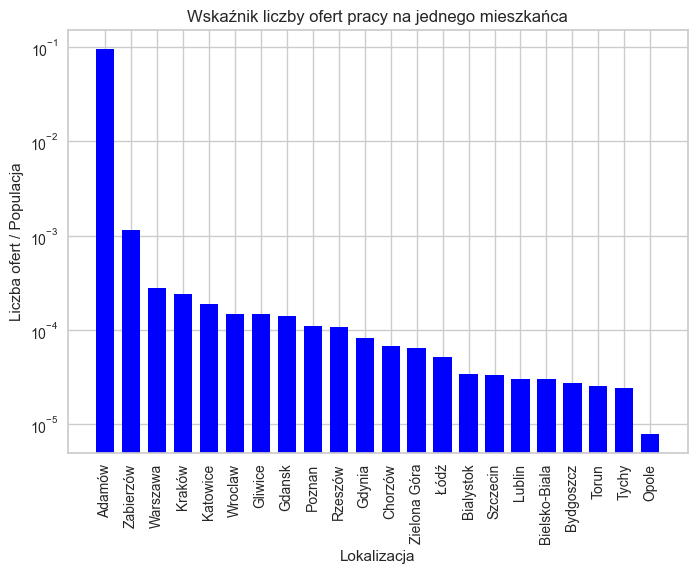
\includegraphics[scale=0.5]{img/location_job_per_pop.png}
\end{center}

Najlepiej mają programiści z Adamowa. Należy jednak wziąć pod uwagę, że Adamów jak i Zabierzów
są bardzo małymi miejscowościami z ulokowanymi w nich firmami informatycznymi ze względu na
bliskość do metropolii odpowiednio warszawskiej i krakowskiej.

Do wizualizacji wskaźnika zastosowano skalę logarytmiczną tak
aby przypadek Adamowa i Zabierzowa nie zaburzał czytelności wykresu.

\subsection{Wstępne oszacowanie}

Wstępnie możemy dokonać analizy zarobków w zależności od potencjanych czynników.

\begin{figure}[!hbt]
    \centering
    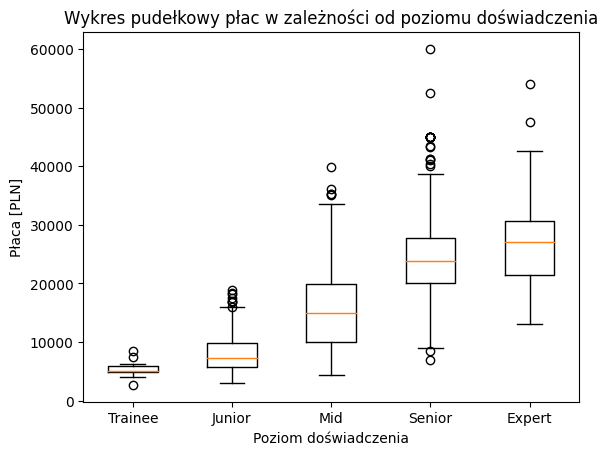
\includegraphics[width=0.7\textwidth]{img/box_zarobki_exp.png}
\end{figure}

\begin{table}[!hbt]
    \centering
    \begin{tabular}{|c|c|}
        \hline
        \textbf{Poziom doświadczenia} & \textbf{Średnie wynagrodzenie [PLN]} \\ \hline
        Expert                        & 26890.65                             \\ \hline
        Senior                        & 24242.49                             \\ \hline
        Mid                           & 15429.12                             \\ \hline
        Junior                        & 8154.89                              \\ \hline
        Trainee                       & 5232.71                              \\ \hline
    \end{tabular}
\end{table}

Z wykresu wynika, że poziom doświadczenia jest wyraźnie skorelowany z wysokością wynagrodzenia co jest zgodne z intuicją.
Im bardziej doświadczony pracownik, tym większą wartość ma jego praca.
Na największe zarobki mogą liczyć programiści klasyfikujący się jako eksperci zaś najmniej jako stażyści i juniorzy.

\begin{table}[H]
    \centering
    \begin{tabular}{|l|c|}
        \hline
        \textbf{Kategoria}    & \textbf{Średnie wynagrodzenie [PLN]} \\ \hline
        Sztuczna inteligencja & 27135.55                             \\ \hline
        Architektura kodu     & 25766.50                             \\ \hline
        Analiza danych        & 23632.85                             \\ \hline
        Agile / Scrum         & 22725.00                             \\ \hline
        Backend               & 21734.63                             \\ \hline
        \dots                 & \dots                                \\ \hline
        HR                    & 10400.39                             \\ \hline
        Marketing             & 8365.63                              \\ \hline
        Prawo                 & 8186.00                              \\ \hline
        Administracja biurowa & 7807.85                              \\ \hline
        Obsługa klienta       & 7166.08                              \\ \hline
    \end{tabular}
\end{table}

\textit{Zarobki od 5-tego miejsca od góry do 5-tego miejsca od dołu zostały pominięte w tabeli dla czytelności.}

\medskip

Na najwyższe zarobki przeciętnie mogą liczyć programiści związani z dziedziną sztucznej inteligencji, architekturą oraz danymi.
Najniższe zarobki przeciętnie otrzymują pracownicy związani z obszarami obsługą klienta, administracją biurową oraz prawem.

\subsection{Korelacja między zmiennymi}

\begin{center}
    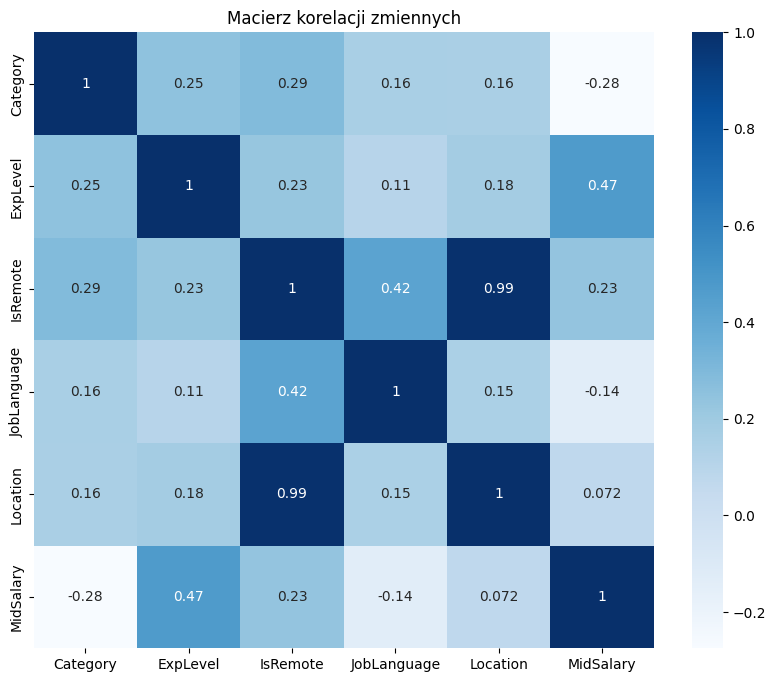
\includegraphics[scale=0.5]{img/corr_matrix.png}
\end{center}

Przy pomocy macierzy korelacji możemy zidentyfikować zmienne, między którymi
istnieje pewna zależność.
Z mapy wynika, że istnieje korelacja między poziomem doświadczenia i wynagrodzeniem. Jest to zgodne z ogólnie przyjętą intuicją,
że im wyższy poziom doświadczenia, tym wyższe zarobki.

Zauważalna jest również korelacja języka (naturalnego) a tym czy praca jest zdalna.
Można spekulować, że wynika to z tego, że język angielski jest wymagany przy współpracy z firmami zagranicznymi,
które nie mając siedziby w Polsce oferują pracę zdalną.

\textit{Korelacja między lokalizacją a pracą zdalną wynika z założenia analizy, że jeśli lokalizacja jest 'Remote' to praca jest zdalna.}
\medskip

Ewentualnymi słabszymi korelacjami, na które można zwrócić uwagę są również:
\begin{itemize}
    \item Praca zdalna a zarobki
    \item Kategoria a praca zdalna
    \item Poziom doświadczenia a praca zdalna
    \item Kategoria a zarobki
\end{itemize}

\section{Opracowanie modelu}

Aby móc odpowiedzieć na pytanie o wpływ czynników na zarobki programistów, należy zbadać ważność poszczególnych zmiennych.
W tym celu najlepiej sprawdzi się model regresji liniowej.
Model regresji liniowej pozwala na przewidywanie wartości zmiennej zależnej na podstawie wartości innych zmiennych.

Poprzez analizę współczynników regresji, można określić, które zmienne mają największy wpływ na zarobki programistów.
Dane zostały podzielone na zbiór treningowy i testowy w stosunku 80:20.
Cechy kategoryczne zostały zakodowane za pomocą kodowania one-hot tak aby model mógł je zinterpretować jako zmienne numeryczne.
Wybór tego kodowania jest podyktowany tym, że zmienne kategoryczne używane w modelu nie mają charakteru porządkowego, model musi
traktować je jako osobne kategorie.

Aby ułatwić zrozumienie przewidywań modelu, niżej przedstawiono grafikę jak należy odczytywać wyniki modelu regresji liniowej na wykresie.

\begin{center}
    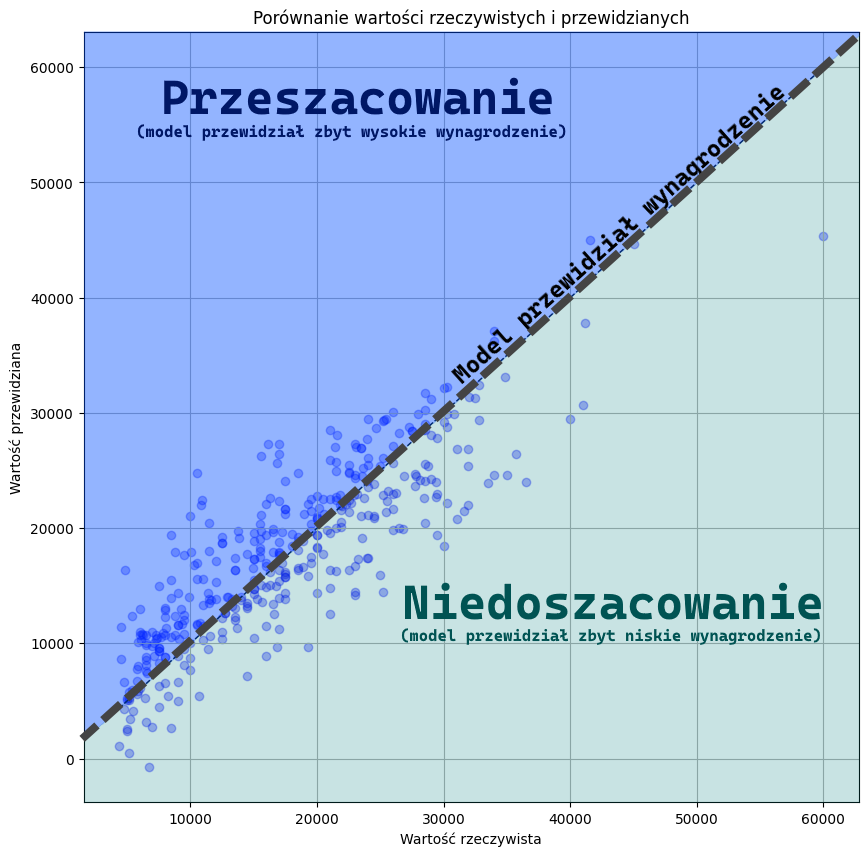
\includegraphics[scale=0.4]{img/czytanie_wykres.png}
\end{center}


\begin{center}
    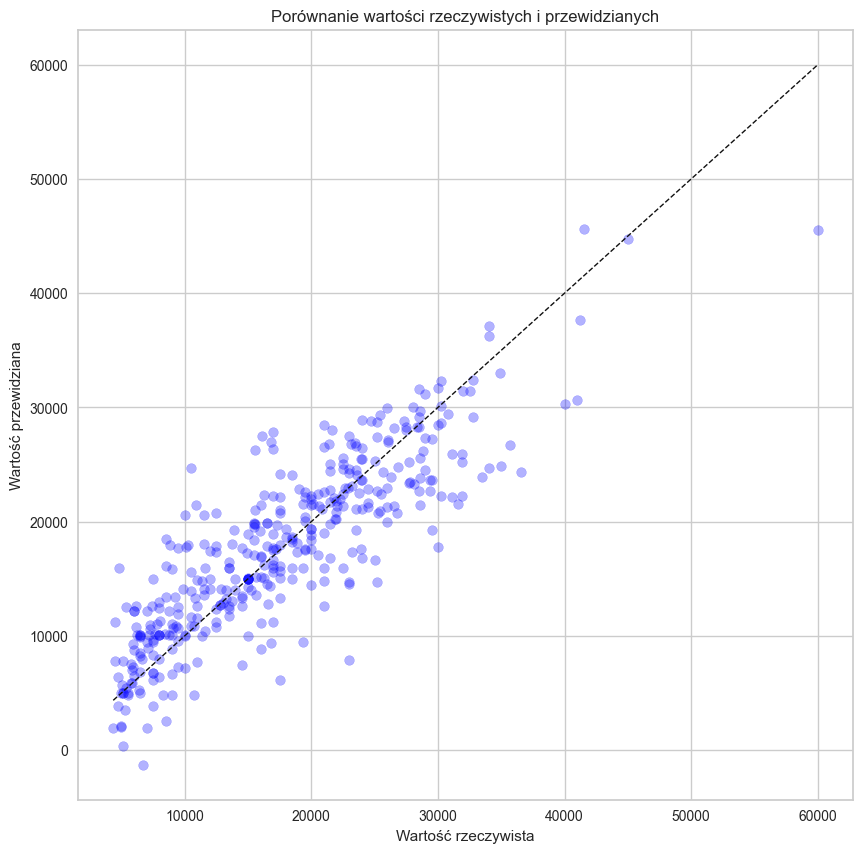
\includegraphics[scale=0.5]{img/model_pred_1.png}
\end{center}

Pod uwagę przy tworzeniu modelu regresji liniowej wzięto następujące zmienne:
\begin{itemize}
    \item Poziom doświadczenia
    \item Technologie
    \item Kategorię branży
    \item Czy praca jest zdalna
    \item Lokalizację miejsca pracy
\end{itemize}

Współczynnik determinacji modelu wynosi 0.73, oznacza to, że model, jest w stanie przewidzieć 73\% zmienności wynagrodzenia przez zmienne objaśniające.

Z wykresu również można zauważyć, że dużo jest ofert pracy, których zarobki nie udało się w pełni przewidzieć.
Różnica między wartościami przewidywanymi a rzeczywistymi w pewnych przypadkach jest bardzo duża - rzędu 10 000 złotych.
Jedną z możliwych przyczyn takiego stanu rzeczy jest brak większej liczby danych w zbiorze bądź atrybutów,
które pozwoliłyby wyjaśnić większą część zmienności zarobków programistów.


\subsection{Ważność zmiennych}

Chcąc rozwiązać problem przewidywania wynagrodzenia programistów należy zidentyfikować zmienne mające
największy wpływ. W przypadku zidentyfikowania tych zmiennych ważną informacją będzie jej kontekst,
czyli analiza na podstawie obserwacji świata rzeczywistego.

\begin{table}[H]
    \centering
    \begin{tabular}{|l|r|}
        \hline
        \textbf{Czynnik}                          & \textbf{Znaczenie} \\ \hline
        (Firma) Snowflake                         & 23646.26           \\ \hline
        (Firma) Technosource                      & 17071.15           \\ \hline
        (Firma) KZ INSPIRE                        & 16624.71           \\ \hline
        (Firma) Chorus One                        & 15690.84           \\ \hline
        (Firma) Infopulse                         & 15651.57           \\ \hline
        (Firma) Plenti                            & 14813.50           \\ \hline
        (Firma) Harvey Nash Technology Sp. z o.o. & 14320.10           \\ \hline
        (Firma) RunBit                            & 12440.59           \\ \hline
        (Firma) vonRoll Infratec.com              & 12315.75           \\ \hline
        (Firma) Be in IT                          & 12208.10           \\ \hline
        (Firma) Transition Technologies PSC S.A.  & 11571.51           \\ \hline
        (Firma) Directio Sp. z o.o.               & 11391.51           \\ \hline
        (Firma) First Derivative                  & 11139.73           \\ \hline
        (Firma) Varwise                           & 10754.25           \\ \hline
        (Firma) Wipro IT Services                 & 10427.30           \\ \hline
        (Firma) int2code GmbH                     & 10255.82           \\ \hline
        (Firma) Consult Red                       & 10077.89           \\ \hline
        (Firma) Tesco Technology                  & 10012.09           \\ \hline
        (Firma) 7N Sp. z o.o.                     & 9839.15            \\ \hline
        (Poziom doświadczenia) Expert             & 9802.32            \\ \hline
    \end{tabular}
    \caption{20 najważniejszych zmiennych w modelu regresji liniowej}
    \label{tab:importance}
\end{table}

Z tabeli wynika, że największy wpływ na zarobki programistów mają zmienne związane z firmą,
z której pochodzi oferta pracy. Ważny przy analizie jest kontekst, gdyż firma z której
pochodzi oferta nie zawsze implikuje wyższych zarobków z faktu, że jest akurat tą firmą.


Duże firmy informatyczne zazwyczaj będą oferowały wysokie zarobki ze względu na swoją renomę,
a co za tym idzie będą chciały przyciągnąć najlepszych pracowników z jak największym doświadczeniem.
Warto mieć to na uwadze przy analizie wyników, chcąc zasugerować się modelem
i zdobyć jak najlepiej płatną pracę osoba powinna się skupić na czynnikach, które są
w większym stopniu od niej zależne.

\bigskip

W celu lepszego zrozumienia czynników wpływających na wygrodzenie, atrybuty powinny zostać
rozdzielone na podkategorie tak, aby móc zobaczyć najważniejsze z nich.

\begin{table}[H]
    \centering
    \begin{tabular}{|c|c|}
        \hline
        \textbf{Poziom doświadczenia} & \textbf{Znaczenie} \\ \hline
        Expert                        & 9802.32            \\ \hline
        Senior                        & 4481.91            \\ \hline
        Mid                           & -394.09            \\ \hline
        Junior                        & -5332.76           \\ \hline
        Trainee                       & -8557.38           \\ \hline
    \end{tabular}
    \caption{Wpływ poziomu doświadczenia na zarobki programistów}
    \label{tab:experience}
\end{table}

Poziom doświadczenia jest cechą, która obejmuje każdego programistę.
Jest cechą, na którą mamy największy wpływ i to ona zawsze będzie czynnikiem,
która będzie wpływać na nasze zarobki. Aby móc lepiej wyciągnąć wnioski z tej cechy można ją
zwizualizować w postaci wykresu.

\begin{figure}[h]
    \centering
    \begin{minipage}{0.45\textwidth}
        \centering
        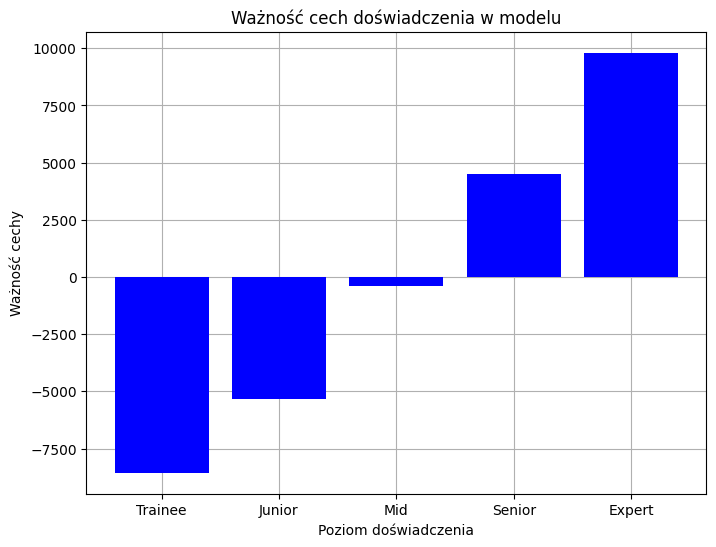
\includegraphics[width=\textwidth]{img/exp_importance.png}
    \end{minipage}
    \hfill
    \begin{minipage}{0.45\textwidth}
        \centering
        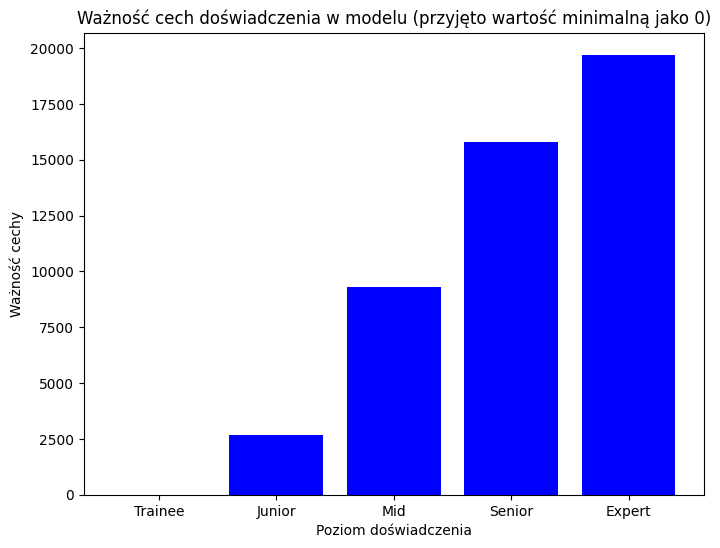
\includegraphics[width=\textwidth]{img/exp_importance_abs.png}
    \end{minipage}
\end{figure}

Im wyższy poziom doświadczenia, tym na wyższe zarobki może liczyć programista.
Warty zauważenia jest fakt, że wzrost wynagrodzenia względem poziomu doświadczenia jest liniowy.

\begin{table}[H]
    \centering
    \begin{minipage}{0.45\textwidth}
        \centering
        \begin{tabular}{|c|c|}
            \hline
            \textbf{Branża}        & \textbf{Znaczenie} \\ \hline
            businessIntelligence   & 5867.84            \\ \hline
            security               & 4827.58            \\ \hline
            artificialIntelligence & 4479.77            \\ \hline
            architecture           & 4054.83            \\ \hline
            projectManager         & 3925.77            \\ \hline
            devops                 & 3510.55            \\ \hline
            erp                    & 3001.52            \\ \hline
            embedded               & 2976.36            \\ \hline
            agile                  & 2909.15            \\ \hline
            data                   & 2818.46            \\ \hline
            frontend               & 2655.47            \\ \hline
            fullstack              & 2378.75            \\ \hline
            telecommunication      & 2152.71            \\ \hline
            backend                & 2098.76            \\ \hline
            businessAnalyst        & 1874.30            \\ \hline
            None                   & 956.40             \\ \hline
            productManagement      & 846.45             \\ \hline
            gameDev                & 446.57             \\ \hline
            sysAdministrator       & 303.16             \\ \hline
            testing                & 50.51              \\ \hline
        \end{tabular}
        \caption{Wpływ branży na zarobki programistów}
        \label{tab:industry}
    \end{minipage}
    \hfill
    \begin{minipage}{0.45\textwidth}
        \centering
        \begin{tabular}{|c|c|}
            \hline
            \textbf{Technologia} & \textbf{Znaczenie} \\ \hline
            Pentesting           & 8680.04            \\ \hline
            CI/CD                & 8624.90            \\ \hline
            Android              & 7992.38            \\ \hline
            iOS                  & 7205.09            \\ \hline
            React native         & 7102.48            \\ \hline
            ORACLE               & 6280.74            \\ \hline
            BeyondTrust          & 6213.83            \\ \hline
            Staking              & 5159.74            \\ \hline
            TPRM                 & 5087.54            \\ \hline
            Selenium             & 4618.72            \\ \hline
            Flutter              & 4395.73            \\ \hline
            k8                   & 4079.92            \\ \hline
            Oracle               & 3586.46            \\ \hline
            CASE                 & 3366.19            \\ \hline
            PixiJS               & 2996.42            \\ \hline
            JasperReports        & 2504.53            \\ \hline
            Kubernetes           & 1832.98            \\ \hline
            Flink                & 1758.12            \\ \hline
            Informatica          & 1651.12            \\ \hline
            GCP                  & 1639.86            \\ \hline
        \end{tabular}
        \caption{Wpływ technologii na zarobki programistów}
        \label{tab:technology}
    \end{minipage}
\end{table}

\section{Oferty bez widełek płacowych}

Ciekawym zagadnieniem jest analiza ofert pracy, które nie zawierają informacji o zarobkach.
Przy pomocy modelu opracowanego na podstawie danych z widełkami płacowymi, można spróbować
przewidzieć zarobki programistów, których oferty nie zawierają tej informacji.
\textbf{Czy oferty pracy bez podanego wynagrodzenia wyróżniają się czymś względem tych, które je posiadają?}

\begin{figure}[h]
    \centering
    \begin{minipage}{0.45\textwidth}
        \centering
        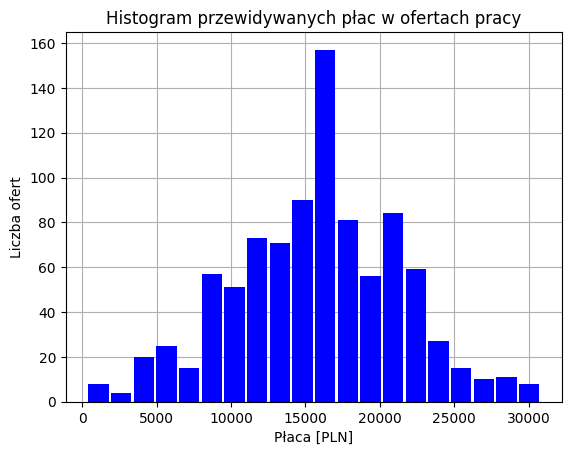
\includegraphics[width=\textwidth]{img/zero_salary_hist.png}
    \end{minipage}
    \hfill
    \begin{minipage}{0.45\textwidth}
        \centering
        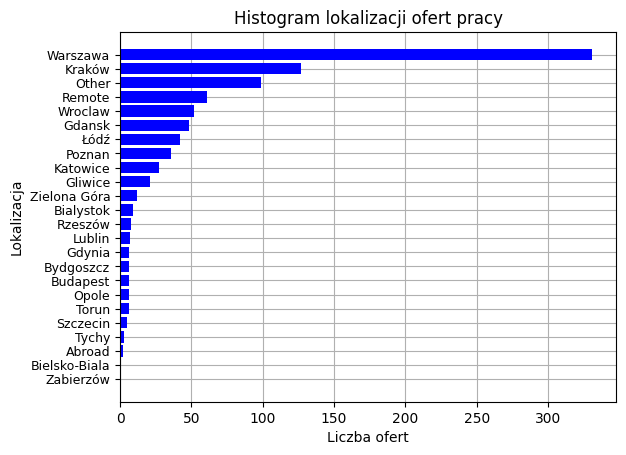
\includegraphics[width=\textwidth]{img/zero_location_hist.png}
    \end{minipage}
\end{figure}

\begin{center}
    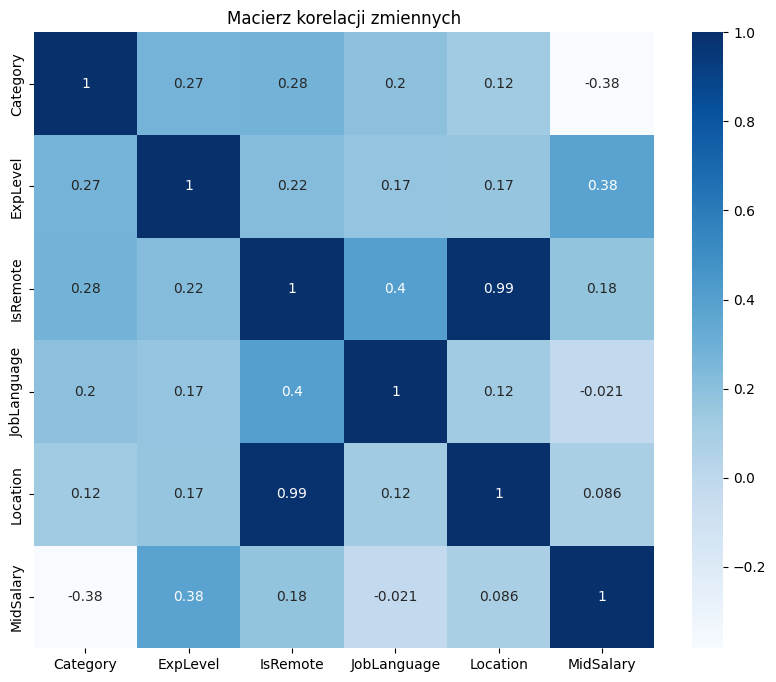
\includegraphics[scale=0.5]{img/corr_matrix_zero_salary.png}
\end{center}

Oferty pracy bez widełek płacowych nie posiadają cech szczególnych w porównaniu do ofert z widełkami płacowymi.
Nie można zauważyć żadnych zależności, dzięki którym moglibyśmy wskazać "w ciemno" czy oferta miała podane wynagrodzenie czy nie.
Przyczyny tego zjawiska mogą być indywidualne dla każdej oferty.

\pagebreak

\section{Wnioski}

Przy pomocy modelu regresji liniowej i macierzy korelacji udało się zidentyfikować czynniki,
które mają największy wpływ na zarobki w branży IT.
Z przeprowadzonej analizy wynika, że największy wpyłw na zarobki mają kolejno:
\begin{itemize}
    \item Poziom doświadczenia
    \item Firma
    \item Technologia
    \item Branża
\end{itemize}

Zauważona została wyraźna korelacja między poziomem doświadczenia a zarobkami, im wyższy poziom doświadczenia,
tym na większe zarobiki może liczyć specjalista IT.

\smallskip

Firma z której pochodzi oferta pracy również ma duży wpływ na zarobki programistów. Im bardziej znana i renomowana firma,
tym wyższe zarobki mogą oferować.
Należy jednak pamiętać, że firma sama w sobie nie gwarantuje wysokich zarobków,
trzeba również wziąć pod uwagę inne czynniki, takie jak poziom doświadczenia czy branża.

\smallskip

W przypadku technologii, największe zarobki związane są z testami penetracyjnymi, CI/CD (tematyka devops), Androidem, iOS oraz React Native.

\smallskip

Jeśli chcemy zarabiać jak najwięcej powinniśmy zainteresować się tematem analizy biznesowej, bezpieczeństwa lub sztucznej inteligencji.
Najniższe zarobki przeciętnie otrzymują programiści związani z testowaniem, administracją systemów czy tworzeniem gier.

\bigskip

Warto zauważyć, że zarobki w branży informatycznej są zróżnicowane i są zależne od wielu czynników, również takich,
które mogły nie zostać uwzględnione w analizie.
Podjęta została również próba zbadania zjawiska ofert pracy bez widełek płacowych, nie udało się jednak
zidentyfikować cech wspólnych wyróżniające te oferty względem ofert z widełkami płacowymi.


\end{document}